\section{History of blockchain}
Early stages of blockchain originate in work of  Stuart Haber and W. Scott Stornetta  in 1991. Their first work involved working on a cryptographically secured chain of blocks whereby no one could tamper with time stamps of documents. They used a hash tree, also called Merkle tree to allow efficient and secure verification of the contents of large data \cite{blockchain_history}. Merkle tree is data-structure in which every leaf node is labelled with the hash of a data block, and every non-leaf node is labelled with the cryptographic hash of the labels of its child nodes. \cite{merkle_tree}

\begin{figure}[H]
    \begin{left}
        \begin{minipage}{\linewidth}
            \begin{left}
                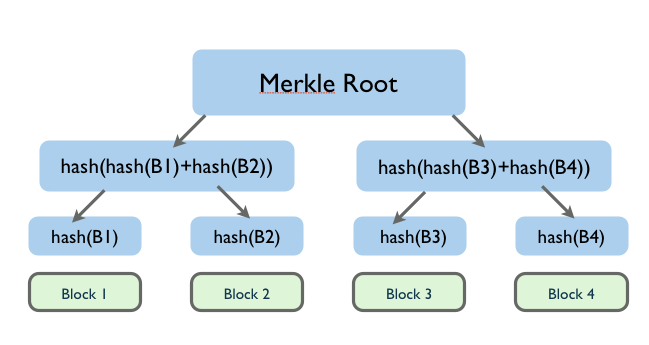
\includegraphics[width=\textwidth,keepaspectratio]{img/blockchain-hash-tree.jpg}
                \caption{Visualisation of Merkle tree}
                \label{obr 1.1.1}
            \end{left}
        \end{minipage}
    \end{left}
\end{figure}

Satoshi Nakamoto, the creator of Bitcoin, claims to be Japanese born in April 1975. It’s unclear whether it’s male or female, single person or a group of people. His or her real identity is well-hidden secret and the main topic of many speculations \cite{satoshi}. 
In 2008, through an online domain \url{bitcoin.org}, the creator of Bitcoin released a white paper. Satoshi outlines how Bitcoin will work using computer networks. The purpose was to eliminate third-party mediators from digital transactions, because of the mediation costs and to remove a single point of failure. Creation of Bitcoin is linked to the financial crisis in 2008. Cause of the crisis were risky loans given out to the people that were unable to pay them back. Multiple banks had to file bankruptcy, and all the money that belonged to the people who trusted the financial institution were lost forever.  
Nakamoto never mentioned blockchain in his first work, he only used words \emph{block} and \emph{chain} separately. Later in 2009, Satoshi Nakamoto released a whitepaper about the technology. In the whitepaper, he described how the technology was well equipped to enhance digital trust given the decentralization aspect that meant nobody would ever be in control of anything. 